% Straight up stealing preamble from Eli Holmes 
%%%%%%%%%%%%%%%%%%%%%%%%%%%%%%%%%%%%%%START PREAMBLE THAT IS THE SAME FOR ALL EXAMPLES
\documentclass{article}

%Required: You must have these
\usepackage{Sweave}
\usepackage{graphicx}
\usepackage{tabularx}
\usepackage{hyperref}
\usepackage{natbib}
%\usepackage[backend=bibtex]{biblatex}
%Strongly recommended
  %put your figures in one place
 
%you'll want these for pretty captioning
\usepackage[small]{caption}

\setkeys{Gin}{width=0.8\textwidth}  %make the figs 50 perc textwidth
\setlength{\captionmargin}{30pt}
\setlength{\abovecaptionskip}{0pt}
\setlength{\belowcaptionskip}{10pt}
% manual for caption  http://www.dd.chalmers.se/latex/Docs/PDF/caption.pdf

%Optional: I like to muck with my margins and spacing in ways that LaTeX frowns on
%Here's how to do that
 \topmargin -1.5cm        
 \oddsidemargin -0.04cm   
 \evensidemargin -0.04cm  % same as oddsidemargin but for left-hand pages
 \textwidth 16.59cm
 \textheight 21.94cm 
 %\pagestyle{empty}       % Uncomment if don't want page numbers
 \parskip 7.2pt           % sets spacing between paragraphs
 %\renewcommand{\baselinestretch}{1.5} 	% Uncomment for 1.5 spacing between lines
\parindent 0pt		  % sets leading space for paragraphs
\usepackage{setspace}
%\doublespacing

%Optional: I like fancy headers
\usepackage{fancyhdr}
\pagestyle{fancy}
\fancyhead[LO]{How do climate change experiments actually change climate}
\fancyhead[RO]{2016}
 
%%%%%%%%%%%%%%%%%%%%%%%%%%%%%%%%%%%%%%END PREAMBLE THAT IS THE SAME FOR ALL EXAMPLES

%Start of the document
\begin{document}

% \SweaveOpts{concordance=TRUE}
 \bibliographystyle{/Users/aileneettinger/citations/Bibtex/styles/nature.bst}
\title{How do climate change experiments actually change climate?} % Paper 1/Large group paper from Reconciling Experimental and Observational Approaches for Climate Change Impacts

\author{A. K. Ettinger,I. Chuine, B. Cook, J. Dukes, A. Ellison, M. Johnston, A.M. Panetta,\\ C. Rollinson, Y. Vitasse, E. Wolkovich}
%\date{\today}
\maketitle  %put the fancy title on
%\tableofcontents      %add a table of contents
%\clearpage
%%%%%%%%%%%%%%%%%%%%%%%%%%%%%%%%%%%%%%%%%%%%%%%%%%%

\section {Aim}

The aim is to write a Concept/Synthesis Paper, for Nature Climate Change, about maximizing benefits of field-based climate change experiments. We argue that there is a need to improve our understanding of how climate is actually altered by these experiments, particularly if we wish to use these experiments to understand biological impacts of climate change. %yann: perhaps also to determine which methods of warming alter the least other climatic variables or to define the most appropriate method regarding the focus of the study (phenology, growth, survival etc)?%annmarie: Somewhere in this paper,  we should discuss that is important that “how” climate variables are modified relative to the predicted change under various emission scenarios is important.  Thus, the “how” should be not only the direction and magnitude of the variable change but also the extent to which the change mirrors change projected for the region in which the experiment took place). build up a discussion of studies that report only mean shifts in temperature in the intro. 

\section {Introduction}
\par Future climate change is expected to cause dramatic changes to Earth's biota. The physiology, distribution, and abundance of organisms will shift, and likely cause cascading community and ecosystem effects \citep{thomas2004,parmesan2006,sheldon2011,urban2012}. Much uncertainty remains about how particular individuals, populations, communities, and ecosystems will respond, making predicting organism responses to the climate change one of the most significant challenges facing biology today.
% EMW: See quick (could be much better) changes below to better handle temperature and precipitation in this paragraph. Much work is on temperature because that's a known, relatively easy to predict effect, at least when compared to precipitation (we may or may not want to sneak this in). 
\par One way that people have sought to understand and forecast future biological conditions is through in situ experimental climate manipulations. Over the past 25 years much focus has been on manipulations to replicated expected higher temperatures. Commonly used field techniques for this include passive warming, such as open-top chambers to increase temperatures, and active warming methods (forced air, soil cables,infra-red radiation). Active warming methods are the most controlled, consistent, and "true to climate change predictions," \citep{aronson2009,wolkovich2012} and we therefore focus on these methods here. In the past XX years, interest has also expanded to understand changing precipitation. Today, many active warming methods are frequently combined with precipitation manipulations, including drought, snow-removal, and supplemental precipitation treatments, in an effort to create climatic conditions such as those forecasted under future climate change scenarios \citep{price1998,cleland2006,sherry2007,rollinson2012}.
% EMW: For the below I would just say 'isolate effect' somewhere clearly. And I would add more of a contrast to OTHER methods (what are the advantage compared to? Long-term data? Data from growth chambers/greenhouses? Modeling studies?). When you have that you should probably add the additional advantage over some other methods of allowing greater climate (especially temperature) and thus the chance to look at important nonlinearities. 
\par Experimental in situ climate manipulations offer several advantages for understanding biological impacts of climate change. Experiments allow temperature and precipitation to be modified in a relatively controlled and rapid way, for example to compare species' performance under current climate conditions versus those forecasted at some future, warmer time \citep[e.g.][]{pelini2014,rollinson2012,jamieson2015}. Field experiments can be performed in places where no historic data exist, so that scientists can understand how a range of climatic conditions affect focal organisms and communities, and are less artificial than ex situ controlled experiments such as greenhouses and laboratory warming chambers.
\par These advantages come at a cost, however. Experimental in situ climate manipulations are logistically challenging and expensive \citep{aronson2009}. It is difficult to design, implement, and monitor replicated experiments that consistently apply the intended climate manipulations, and multiple climatic variables may be affected by these manipulations, beyond the target ones. 
Furthermore, these manipulations often include detailed monitoring of climate variables, yielding large amounts of data, such as daily, or even hourly temperature and other climate variables, over the course of the experiment. Scientists, however, rarely present the results of these detailed data---most publications report only the mean change in climate over the course of the experiment and whether or not that mean change matched their target level of change \citep{price1998,clark2014a,clark2014b,rollinson2012}. 
\par The focus on biological responses to mean shifts makes sense, at least as a first pass at understanding how species respond to warming or other climatic changes. However, as we seek to prepare for future, altered conditions in our biological environment, scientists and others often wish to extrapolate the results of these in situ climate change experiments to forecast how organisms and ecosystems will respond to particular climate change scenarios. 
% EMW: above sentence is great! May want to work text so it is a topic sentence.
Even in cases when this is not the explicit goal of warming and other climate change experiments, it would be incredibly useful to be able to apply knowledge gained from these experiments to improve our understanding and forecasting of how anthropogenic warming will affect species' performance (growth, survival) and distributions. Our ability to make this application is currently limited because a detailed assessment of exactly how experimental warming treatments alter climate, beyond mean differences, and the extent to which these manipulations accurately model the real world, both present and future, are lacking. 
\par Here, we suggest that a more nuanced understanding of how climate change experiments actually change climate is critical if we wish to realize the forecasting potential of climate change experiments. We first use plot-level microclimate data from 10 climate change experiments that manipulate temperature (and precipitation, in some cases) to demonstrate the complex ways that climate is altered by active warming treatments, both directly and indirectly. We then discuss the challenges of interpreting biological implications of experimental shifts in climate, when these climate manipulations are more complex then simple shifts in the mean. Finally, we make recommendations for future climate change experiments.
% EMW: This:
% We use these data, as well as experience gained from XX years of combined experience on the part of the authors in field-installed in situ experimental warming...
% sounds more like cover letter material than for the main text.

\section {Complications in extrapolating experimental climate change}
Climate change experiments often collect detailed microclimate data, at the plot level. However, biologists are generally interested primarily in the biological responses associated with each treatment (e.g. growth or abundance of a species). Not surprisingly then, authors typically report the mean change in temperature, humidity, or other climatic factor achieved under different treatments, and provide more detailed information on the observed biological responses. The imposed climate manipulations result in much more than a simple shift in the mean, however.
\subsection {Treatments Vary Over Time}
There is often temporal variation in applications of experimental warming, and this variation may be divergent from real (i.e. non-experimental) temperature patterns so it should carefully be considered in extrapolating experimental warming to future climate change impacts. Add details and examples of why this occurs, since warming experiments are tied to ambient conditions. 
\begin{itemize}
\item There are frequently strong seasonal variations in experimental warming effects (Figure 1). This can occur because treatments are not applied consistently over the year, either because heat applications are frequently shut off during some seasons such as when snow cover is present \citep[e.g.][]{clark2014a,clark2014b} (Austria,Norway studies) or because some heating methods, even if left on throughout the year, are not capable of applying consistent warming year-round (e.g. infrared radiation, CITATION). Furthermore, seasonal precipitation patterns can alter the effectiveness of warming treatments. % it is likely that this would yield different effects than if heating were turned on during winter (because then you change soil nutrient mineralization which might be important in winter and so change nutrient availability and moisture for the growing season ).

 \begin{figure}[p]
     \centering
 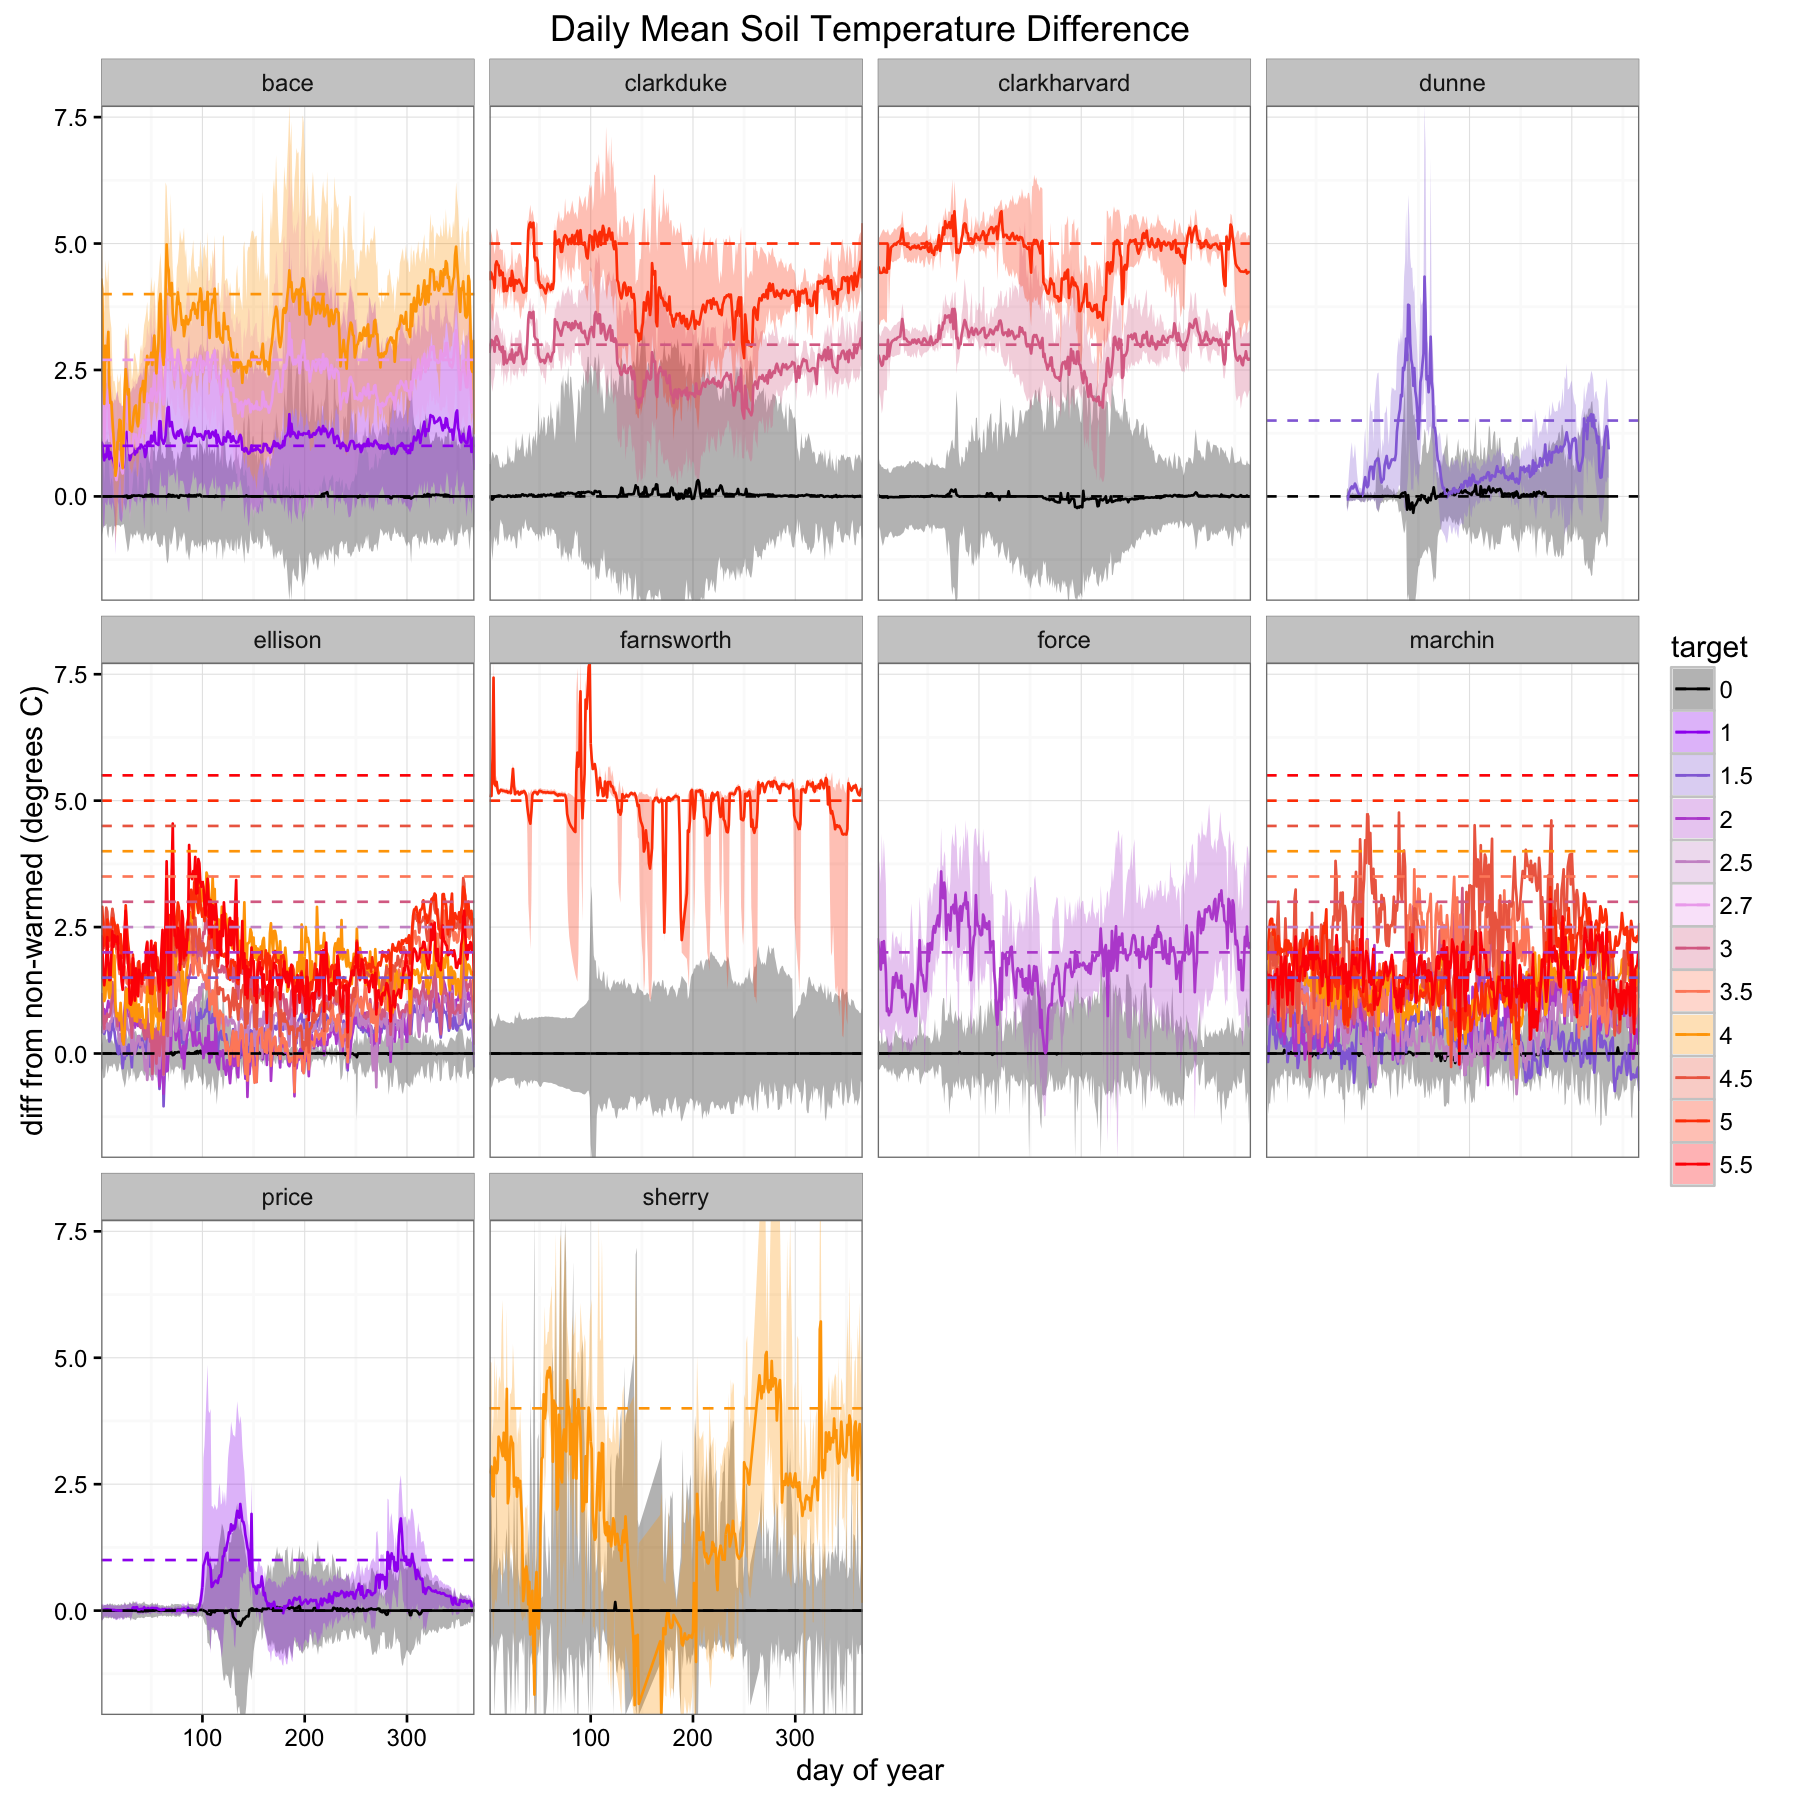
\includegraphics{figures/Exploratory_TimeSeries_SoilTemp1Mean_Deviation.png}    
 \caption{Time series of deviations from mean soil temperature over one year, in control (black line) and warming treatments with various target warming levels at 10 study sites.}
 \end{figure}
\item In addition to seasonal patterns, experimental warming effects can vary on a daily timescale. %could add figure of tmin vs Tmax vs. Tmean. 
It is common to report only the daily mean temperature, however, this may hide huge variations in minimum and maximum temperatures. %there are several recent papers showing the importance of diurnal over nocturnal temperature on phenology.
\item Anne Marie- please add a paragraph on your suggested discussion "that 3-5 year studies may not capture ultimate, long-term responses that may actually be in the opposite direction to short-term responses.  Cite recent Global Change Biology paper by Harte et al.  Ideally, we want to run studies long enough to capture population-level responses to warming." 
\end{itemize}
\subsection {Treatments Vary in Space}
There is spatial variation in experimental warming effects, such that extrapolation of experimental warming to forecast climate change impacts may not be a straightforward space-for-time substitution. Presumably there will also be spatial variation in climate change effects.  Accurate extrapolation may therefore depend on the extent to which experiments encompass a representative amount of existing natural variation (e.g. gradients in slope, aspect, etc) present at the scale at which the extrapolation is being made. From Aaron: "most space-for-time substitutions turn out to be inaccurate. I think because we make assumptions about state of assemblages and temporal stationarity that are unrealistic." (Add citations about this?)
\begin{itemize}
\item Analysis of plot vs. block level variation vs. treatment effects. Lizzie is working on this.
\item Documented variation in warming within plots (i.e. edge effects)? (This is known for open-top chambers)
\end{itemize}

\subsection {Experimental Infrastructure Alters Climate}
The experimental structures themselves alter temperature and other important biotic and abiotic variables, in ways that are not generally examined or reported in experimental warming studies. The possible existence of these effects are widely acknowledged, and many studies include "shams" or "disturbance controls" to account for them. However, the magnitude of structural effects on climate are rarely discussed, accounted for, or interpreted in climate change studies.
% EMW: Explain below why these studies? I assume they are the only ones with these shams and such, right? If so, we should say that. 
\par To investigate the magnitude of these effects, we compared temperature and soil moisture data from four active warming studies at two sites (Duke Forest and Harvard Forest, Farnsworth et al, Clark et al, Ellison et al, Marchin). These studies included two types of control plots: structural controls (i.e. "shams" or "disturbance controls," which contained all the warming infrastructure, such as soil cables or infrared heating units but with no heat applied) and ambient controls with no infrastructure added (see Supplement for detailed methods).  

\par We were surprised to find that experimental structures altered air and soil temperatures in opposing ways:  air temperatures were higher in the structural controls, compared with the ambient air with no structures installed, whereas soil temperatures were lower in the structural controls compared with ambient soil (Figure 1). This was consistent across the different temperature models we fit (monthly mean, minimum, and maximum), and the sign of the effects was consistent across study-sites and months, although the magnitude varied among sites (Table 1) and across the year (Figure 1). Soil moisture was lower in structural controls compared with ambient conditions (Figure 1S). In addition to these documented effects, experimental structures may alter conditions by creating shade, intercepting precipitation, and altering herbivory and other biotic interactions. %EMW: Needs more here.

 \begin{figure}[p]
     \centering
 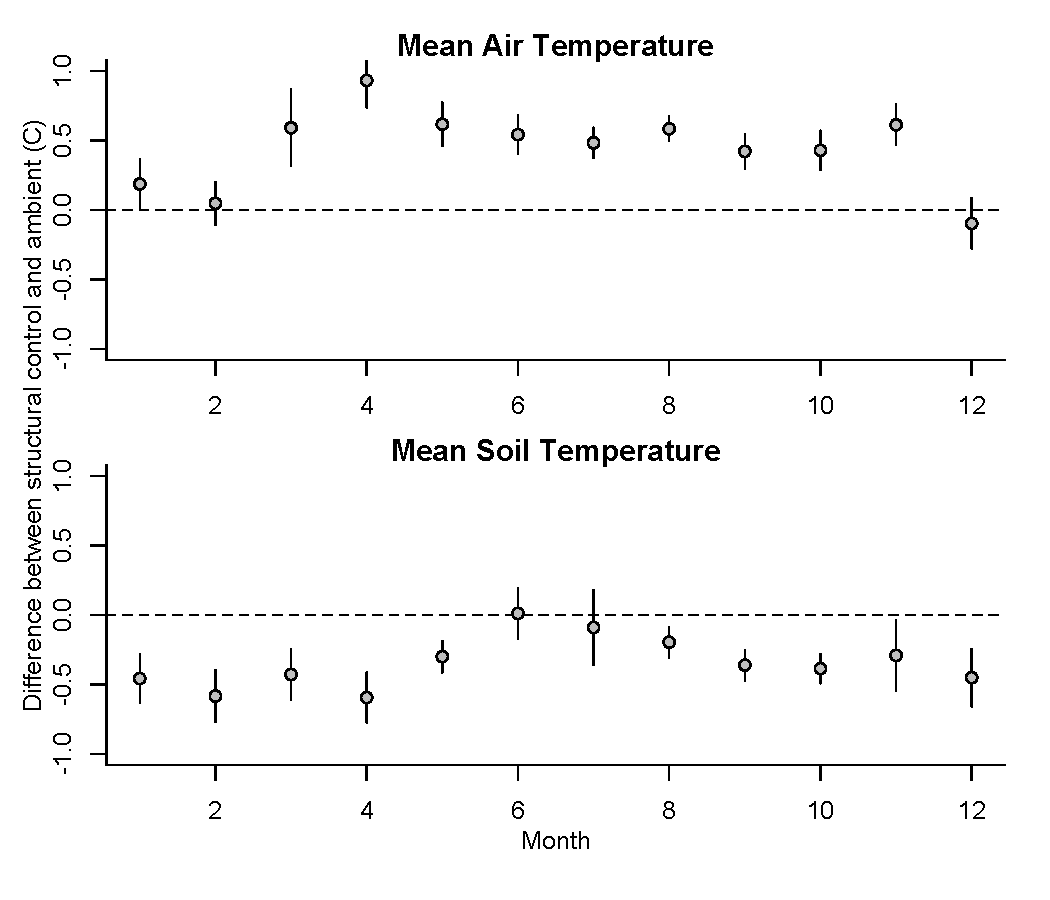
\includegraphics{figures/ShamVSAmbient_mean.pdf}    
 \caption{Difference between mean air and soil temperatures in structural controls compared with ambient controls, with no control chambers or warming infrastructure in place. Air temperatures were higher, whereas soil temperatures were lower in the structural controls compared with ambient conditions. We show fixed effects from a mixed effects model that accounts for differences in experimental design and other factors among sites by including site as an intercept-only random effect (see shamvambient.R for details). }
 \end{figure}

\section {Secondary Effects of climate change manipulations}
Climate change experiments often manipulate one or two variables, such as temperature and precipitation. However, as scientists who have conducted these experiments have likely experienced, climatic variables are nearly impossible to completely isolate from one another.  Temperature, for example, interacts with precipitation to alter the abiotic environment: Rollinson et al (2012) observed that a twenty percent increase in precipitation reduced mean hourly temperatures by 0.3 degrees Celsius over the course of their two-year experiment. Ideally, experimentally induced changes in other variables would be realistic; for example, the experimental treatment should not increase moisture in an area projected to get much drier. At the very least, it is important to quantify the secondary effects of applied manipulations.  Understanding the effects of an experimental treatment on the suite of interrelated variables is critical when one is trying to determine mechanistic explanations for observed responses to warming.
\begin{itemize}
\item Effects of precipitation on temp (BACE, Rollinson)

\item Effects of experimental warming on air humidity (use Isabelle's data?). This affects VPD with potential impact for stomata closure (paper out on this response (sapflow, vpd) from Pam Templer's group using Harvard Forest ant warming chambers effects on oak trees)
\item Change in biotic interactions: if warming increase the abundance and composition of species it might change competition for resources...
\end{itemize}
\section {Biological Implications}
\par We have highlighted a suite of factors that complicate   interpretation of warming experiments. We argue that these largely unintended alterations are important for scientists to fully understand and report in their research because they are likely to have biological implications (Figure 3).
\par Examples:
\begin{itemize}
\item Plant phenology: likely to be altered in opposing ways by
the increased air temperatures and decrease soil moisture, cite Wolkovich et al's earlier work finding discrepancy between observation and experimental phenology responses to warming. (Aaron: plants also respond to variability, perhaps more than mean, as we saw in W Mass this year with fruit tree flowering)
\item Soil respiration or other microbe studies? (tight link between microbial activity and plant growth under warming. net mineralization should be accounted for)
\item Plant growth- photosynthesis and transpiration are likely to be altered in opposing ways by the increased air temperatures and decrease soil moisture/temperature %Lizzie: I think you could find simple references in Larcher or another basic plant physiology book (Terry Chapin's?) to small temperature changes having a big effect. aforementioned paper by Templer group (Ecosphere 2016) may be a useful example. Paper here: http://harvardforest.fas.harvard.edu/sites/harvardforest.fas.harvard.edu/files/ellison-pubs/2016/Juice_etal_2016_Ecosphere.pdf
\item change in biotic interactions (see previous comment): both plant-plant and microbes/fungi-plants
\item intraspecific variation? All plants, ants, microbes, etc. of a single species not equivalently responsive. 
\item herbivory
\end{itemize}
 \begin{figure}[p]
     \centering
 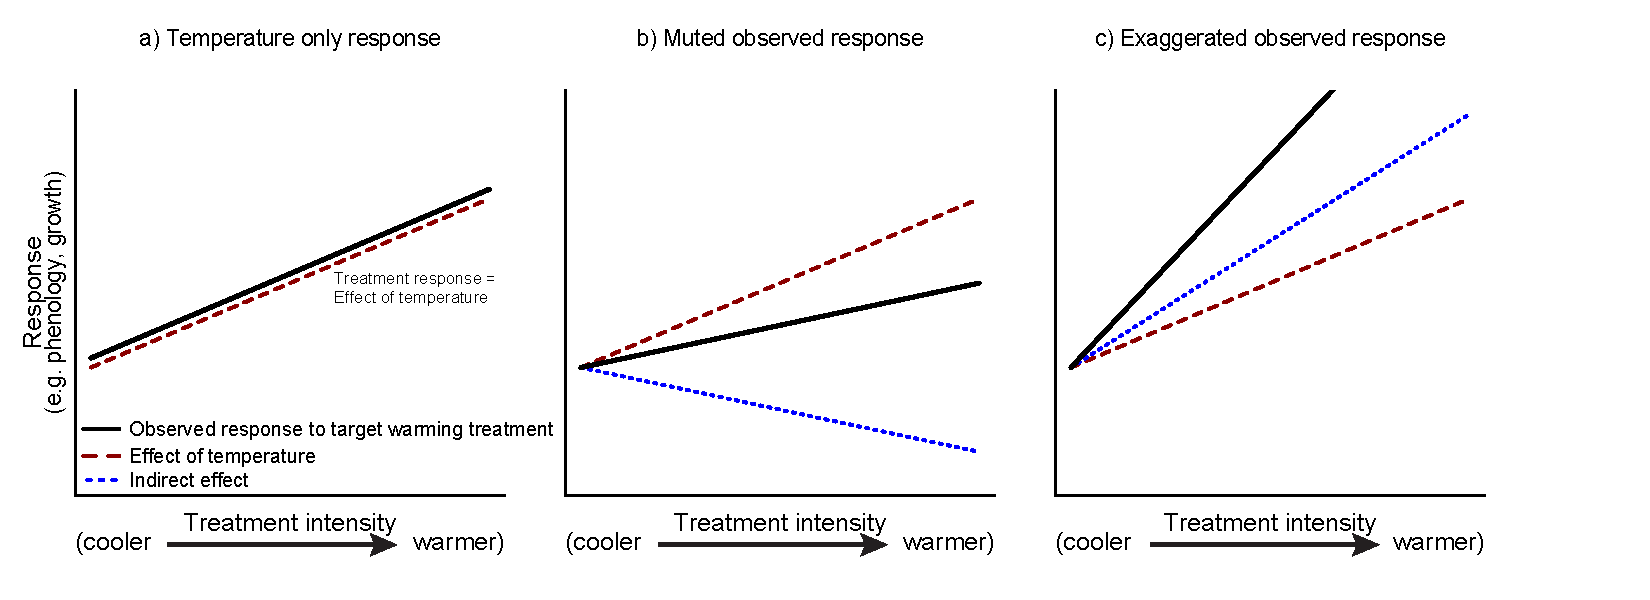
\includegraphics{figures/DirIndWarmingEffects.pdf}    
 \caption{Experimental warming may cause biological responses to be muted or exaggerated, compared to direct responses to temperature alone, when indirect effects of experimental warming are also drivers of focal responses. For example, phenology may appear to be less sensitive to warming in experiments versus observational studies \citep{wolkovich2012} because experimental warming reduces soil moisture, perhaps more than natural warming.}
 % EMW: Change the Y axis title so it's clearer -- effect of structural control (difference ....)?
 \end{figure}
\section {Recommendations for future climate change experiments}
 \par The complications of climate change experiments that  we describe are not meant to be criticisms or to imply that experimental climate change studies are not worthwhile. On the contrary, we believe that climate change experiments provide invaluable information about biological responses to climate change.
 We believe that we need to more fully explore the ways in which these warming experiments are altering climate, as it is clearly not simply shifting the mean. Here we describe a few recommendations to improve implementation, interpretation, and communication of future climate change experiments.
\begin{itemize}

\item Prior to experimental setup, consult climate change projections for the study region.  Pick a warming/precipitation treatment method that most accurately mimics anticipated changes. Or at the minimum, report how your study compares to projected changes. 
\item Include structural and ambient controls, and collect, use, and report data collected within them in. 
\item Run experiments for as long as possible. Climate change experiments should run for several seasons to account for the inter-annual variations that may interact with the warming treatment itself (especially when looking at non linear processes such as phenology), and to capture more than transient responses.
 \item Collect climate data at least twice daily, and ideally hourly. 
\item Carefully consider and report the timing of warming treatment applied.
 \item Publish high quality, usable data and metadata. In the metadata, report the number and cause of missing data points for climate, especially those collected in warming treatments. (For example, are data missing because the heaters went out, or because rodents at the sensors?) Also report the timing of applied warming treatments (i.e. exact start and end dates, within and across years), as well as variations in daytime and nighttime and season variations in climate variables. 
\item Consider implementing and following community standards for reporting climate data (and phenology -Chuine et al. 2017) %EMW: Do we have community standards for climate data? Someone must .... and we should ask Ben if he has any ideas of resources for this. 

 \end{itemize}
%Notes from Aaron, who doesn't think that pooling the plots makes sense. (I should explain that I used mixed effects models with random effect of site to account for this):There are some big differences in exps that are obscured by pooling in these plots. Because of that, pooling them doesn't make sense to me.Farnsworth is soil-warming cables only Clarkduke & Clarkharvard are soil warming cables + air heating, but air heating is turned off in winter at Harvard (not sure about Duke) while cables (I think) were left on.
% ellison and marchin are air warming only, run all year.below, it seems as though we should mention ( in this section and perhaps even in the intro) that these recommendations stem from an attempt to gather and analyze data from many warming experiments.  We could make some sort of statement about how important it is, when trying to understand implications of a global challenge as large as climate change, that we design, run, and report experiments in such a way that we may eventually give rise to a global dataset.

\section{Supplemental Information}

To account for differences in the type of warming and other unmeasured site/study differences (e.g. forced air for Ellison and Marchin; heating cables for Farnsworth and ??), we fit linear mixed effects models with random effect of study-site. Response variables were daily soil or air temperature (models with daily  mean, minimum, and maximum were all fit) and , and the explanatory variable was control type (infrastructure or ambient). We used a random slopes and random intercepts structure, so that the effect of control type, as well as the mean temperature, were allowed to vary across study-sites. We fit models across the entire year, as well as separate models for each month to examine if effects varied seasonally.

\bibliography{/Users/aileneettinger/citations/Bibtex/mylibrary}

%%%%%%%%%%%%%%%%%%%%%%%%%%%%%%%%%%%%%%%%
\end{document}
%%%%%%%%%%%%%%%%%%%%%%%%%%%%%%%%%%%%%%%%
